\subsection{COXETER MATRICES AND COXETER GRAPHS}

DEFINITION 4. Let I be a set. A Coxeter matrix of type I is a symmetric square matrix \(\mathrm{M} = (m_{ij})_{i,j\in \mathrm{I}}\) whose entries are integers or \(+\infty\) satisfying the relations

\[
m _ {i i} = 1 \quad \text {   for   all   } i \in \mathrm{I};\tag{25}
\]

\[
m _ {i j} \geqslant 2 \quad \text {   for   } i, j \in I \text {   with   } i \neq j.\tag{26}
\]

A Coxeter graph of type I is (by abuse of language) a pair consisting of a graph \(\Gamma^{3}\) having I as its set of vertices and a map f from the set of edges of this graph to the set consisting of \(+\infty\) and the set of integers \(\geqslant 3\) . \(\Gamma\) is called the underlying graph of the Coxeter graph \((\Gamma, f)\) .

A Coxeter graph \((\Gamma, f)\) is associated to any Coxeter matrix \(M\) of type I as follows:

the graph \(\Gamma\) has set of vertices I and set of edges the set pairs \(\{i,j\}\) of elements of I such that \(m_{ij} \geqslant 3\) , and the map \(f\) associates to the edge \(\{i,j\}\) the corresponding element \(m_{ij}\) of M.

It is clear that this gives rise to a bijection between the set of Coxeter matrices of type I and the set of Coxeter graphs of type I.

To assist the reader in following our arguments, we often represent a Coxeter graph of type I by the diagram used to represent its underlying graph, and write either next to or above each edge \(\{i,j\}\) the number \(f(\{i,j\})\) . We generally omit these numbers if they are equal to 3.

If (W,S) is a Coxeter system, the matrix \(M = (m(s,s'))_{s,s' \in S}\) , where \(m(s,s')\) is the order of \(ss'\) , is a Coxeter matrix of type S which is called the Coxeter matrix of (W,S): indeed, \(m(s,s) = 1\) since \(s^2 = 1\) for all \(s \in S\) , and \(m(s,s') = m(s',s) \geqslant 2\) if \(s \neq s'\) since \(ss' = (s's)^{-1}\) is then \(\neq 1\) . The Coxeter graph \((\Gamma, f)\) associated to M is called the Coxeter graph of (W,S). We remark that two vertices \(s\) and \(s'\) of \(\Gamma\) are joined if and only if \(s\) and \(s'\) do not commute. For example, the Coxeter matrix of a dihedral group of order \(2m\) is \(\begin{pmatrix} 1 & m \\ m & 1 \end{pmatrix}\) and its Coxeter graph is represented by

when \(m \geqslant 3\) (or

\pandocbounded{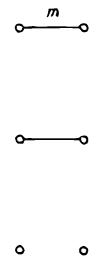
\includegraphics[keepaspectratio]{images/part001_5ff7a109.jpg}}

if \(m = 3\) ) and by

when \(m = 2\) . *The Coxeter graph of the symmetric group \(\mathfrak{S}_n\) is represented by

\pandocbounded{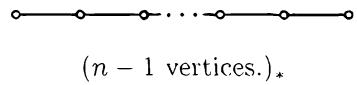
\includegraphics[keepaspectratio]{images/part001_1071b0ee.jpg}}

We show later (Chap. V, §4) that, conversely, any Coxeter matrix is the matrix of a Coxeter system.

A Coxeter system \((W,S)\) is said to be irreducible if the underlying graph of its Coxeter graph is connected (Appendix, no. 2) and non-empty. Equivalently, S is non-empty and there exists no partition of S into two distinct subsets \(S'\) and \(S''\) of S such that every element of \(S'\) commutes with every element of \(S''\) . More generally, let \((\Gamma_{i})_{i\in I}\) be the family of connected components of \(\Gamma\) (Appendix, no. 2) and let \(S_{i}\) be the set of vertices of \(\Gamma_{i}\) . Let \(W_{i}=W_{S_i}\) , be the subgroup of W generated by \(S_{i}\) (cf.~no. 8). Then the \((W_{i},S_{i})\) are irreducible Coxeter systems (no. 8, Th. 2) called the irreducible components of \((W,S)\) . Moreover, the group W is the restricted direct product \(^{4}\) of the subgroups \(W_{i}\) for \(i\in I\) . Indeed, this follows from the following more general proposition:

PROPOSITION 8. Let \((\mathrm{S}_{i})_{i\in\mathrm{I}}\) be a partition of S such that every element of \(S_{i}\) commutes with every element of \(S_{j}\) if \(i\neq j\) . For all \(i\in I\) , let \(W_{i}\) be the subgroup generated by \(S_{i}\) . Then W is the restricted direct product of the family \((\mathrm{W}_{i})_{i\in\mathrm{I}}\) .

It is clear that for all \(i \in I\) the subgroup \(W_i'\) generated by the union of the \(W_j\) for \(j \neq i\) is also generated by \(S_i' = \bigcup_{i \neq j} S_j\) . Thus

\[
\mathrm{W} _ {i} \cap \mathrm{W} _ {i} ^ {\prime} = \mathrm{W} _ {\varnothing} = \{1 \}
\]

by Th. 2 of no. 8. Since W is generated by the union of the \(W_{i}\) , this proves the proposition.

